% http://cds.cern.ch/record/2801878/files/document.pdf?version=1
% https://iopscience.iop.org/article/10.1088/1748-0221/16/04/C04004
% https://twiki.cern.ch/twiki/bin/view/Main/EndcapReshufflingRpc

The CMS Resistive Plate Chambers (RPCs) are a group of 1056 chambers placed in both the CMS barrel and endcap sections for muon detection, filled with a gas mixture of $C_{2}H_{2}F_{4}$, $C_{4}H_{10}$ and $SF_{6}$. In a fashion similar to the CSCs, the RPCs detect muons via direct ionization of its gaseous mixture. The layout of an RPC module is shown in Figure \ref{fig:RPC_Schema}. 

\begin{figure}[H]
    \centering
    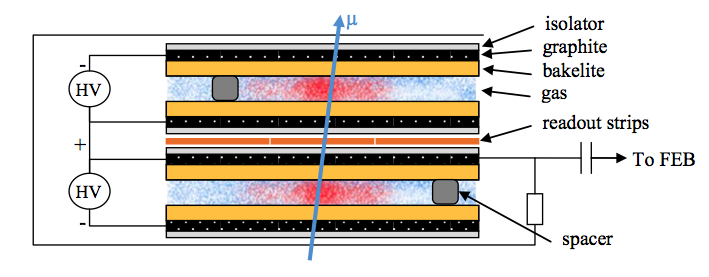
\includegraphics[width=0.9\textwidth]{Images/CMS/Muons/RPC/RPC_Schema.png}
    \caption{RPC schematic.}
    \label{fig:RPC_Schema}
\end{figure}

The idea behind the geometry of an RPC chamber is to have readout strips in the center, with gaseous chambers located on either side. 

Like the CSCs, throughout Run 2 the RPCs maintained excellent hit efficiency, as shown separately for the barrel and endcap portions in Figures \ref{fig:RPC_Barrel_Eff} and \ref{fig:RPC_Endcap_Eff}. 

\begin{figure}[H]
    \centering
    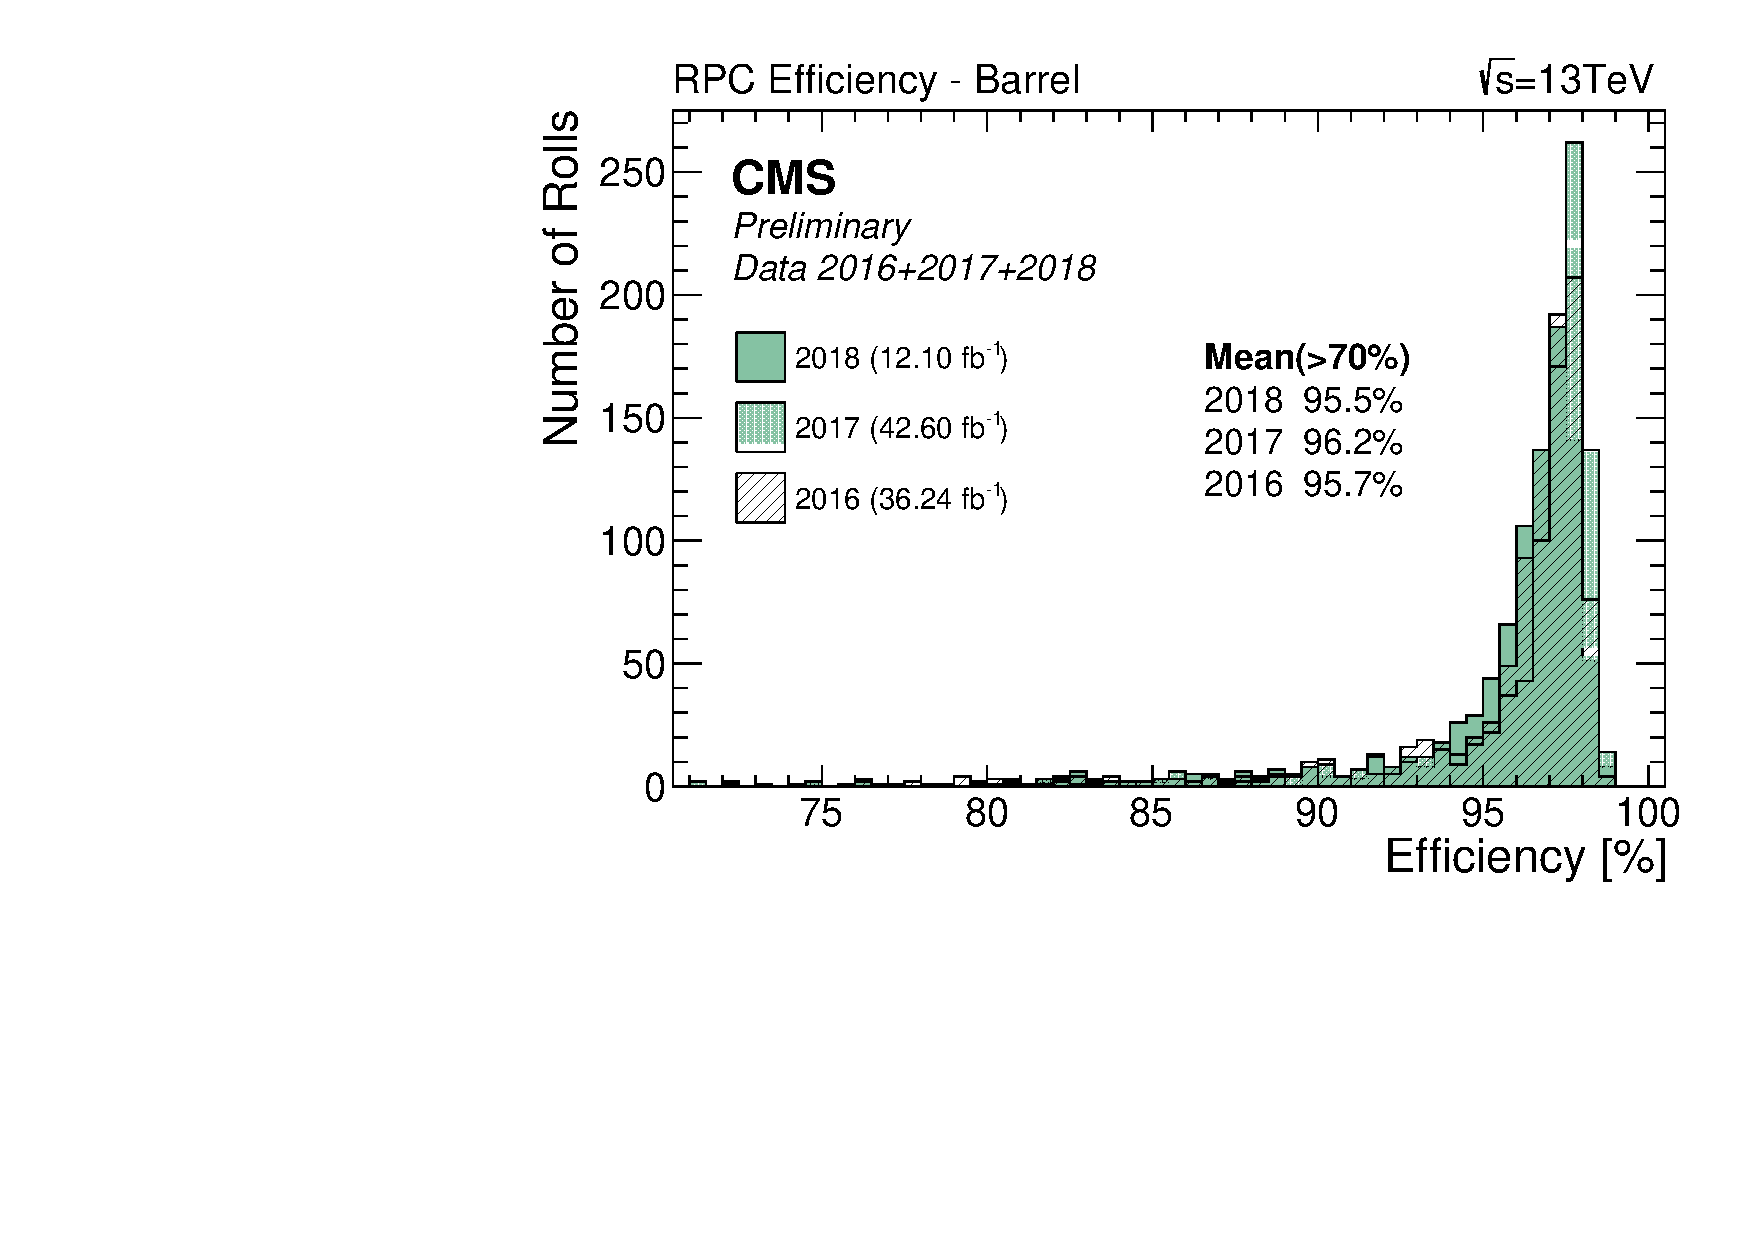
\includegraphics[width=0.7\textwidth]{Images/CMS/Muons/RPC/RPC_EffCmpBarrel.pdf}
    \caption{RPC barrel efficiency during LHC Run 2.}
    \label{fig:RPC_Barrel_Eff}
\end{figure}

\begin{figure}[H]
    \centering
    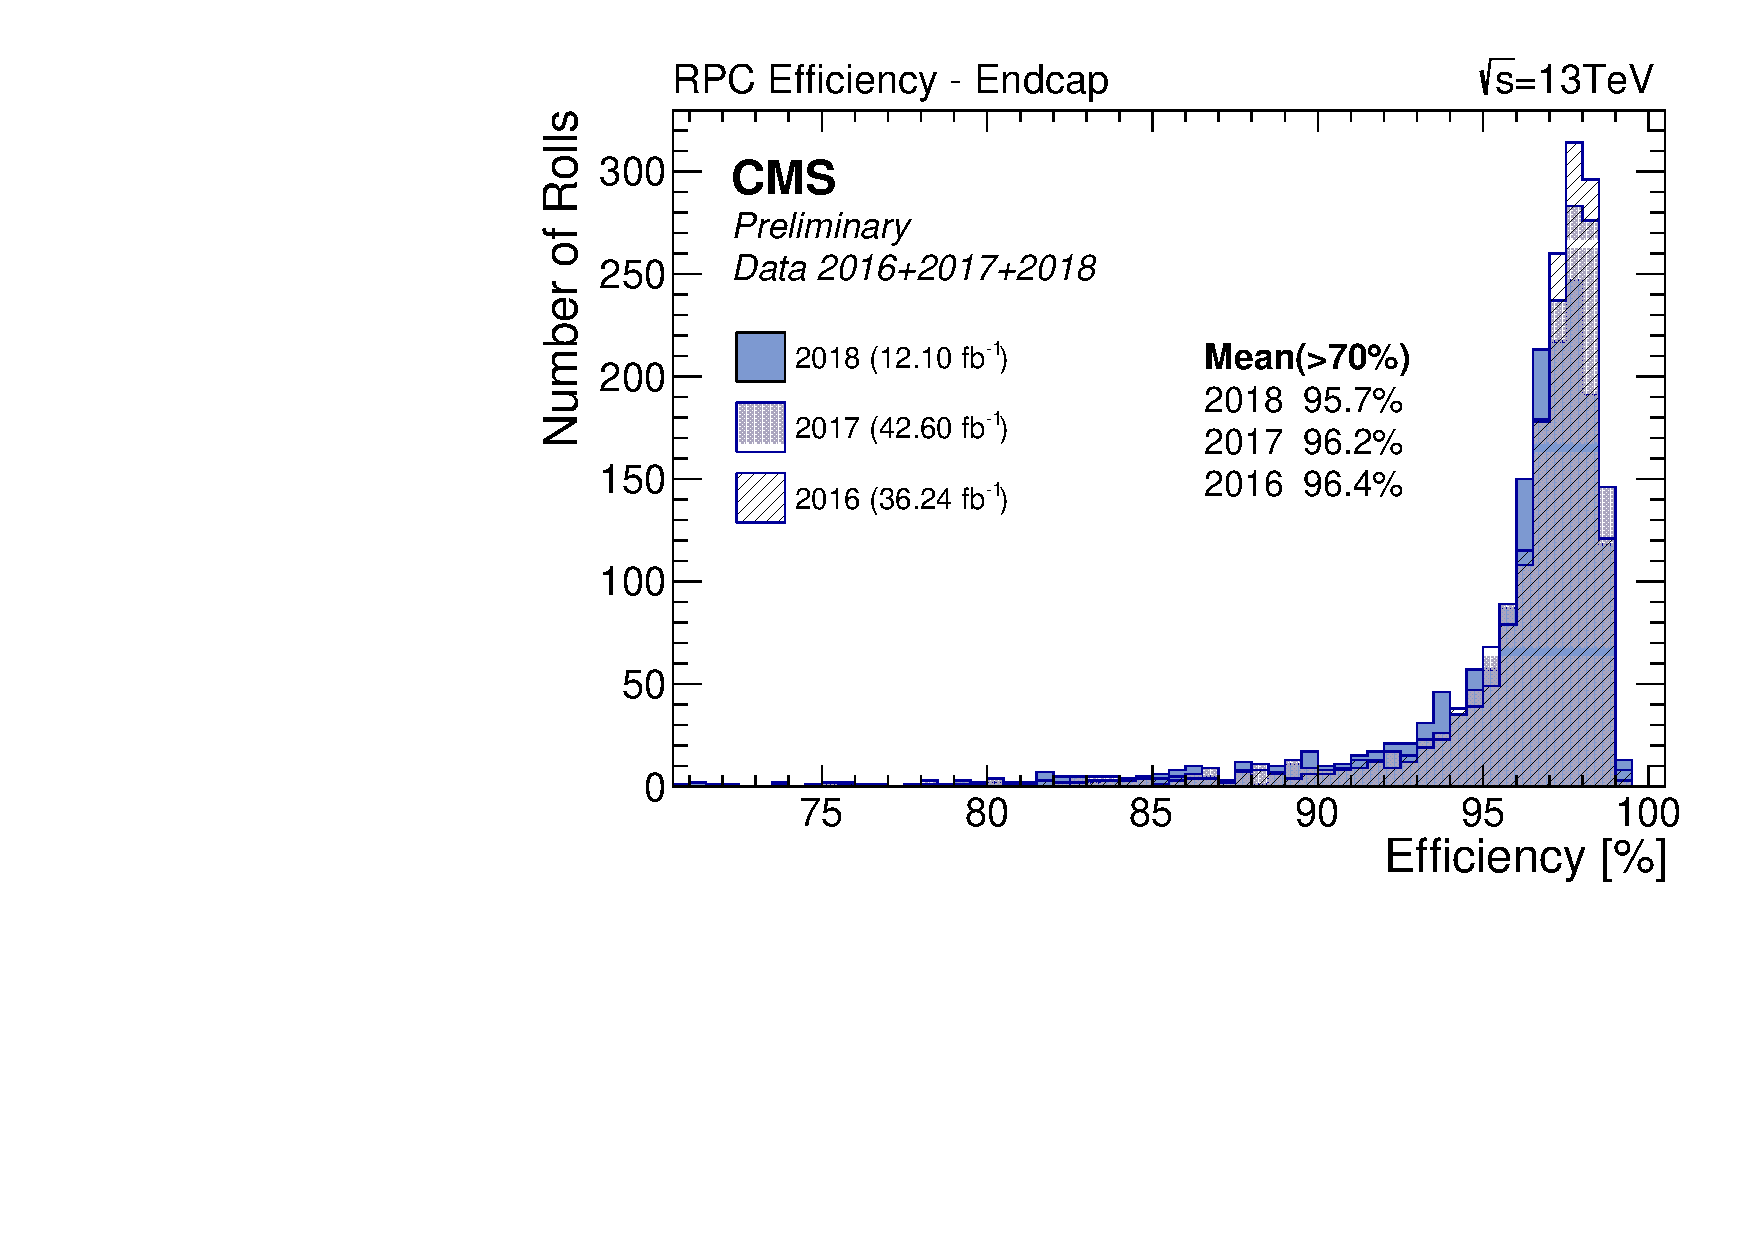
\includegraphics[width=0.7\textwidth]{Images/CMS/Muons/RPC/RPC_EffCmpEndcap.pdf}
    \caption{RPC endcap efficiency during LHC Run 2.}
    \label{fig:RPC_Endcap_Eff}
\end{figure}

